\documentclass[a4paper,11pt]{article}

\usepackage[T1]{fontenc}
\usepackage[utf8]{inputenc}

\usepackage{multirow}
\usepackage{booktabs}
\usepackage{graphicx}
\usepackage{setspace}
\usepackage[skip=6pt plus1pt, indent=0pt]{parskip}

\usepackage{float}
\usepackage{fancyhdr}

\usepackage{tcolorbox}
\usepackage{hyperref}
\hypersetup{
    colorlinks=true,
    linkcolor=blue,
    filecolor=magenta,
    urlcolor=blue
}

\usepackage[margin=1in]{geometry}

\newcommand{\incode}[1]{
\begin{tcolorbox}[colback=blue!5!white, boxrule=0mm, sharp corners]
\texttt{#1}
\end{tcolorbox}
}

\newcommand{\note}[1]{\textit{\textcolor{gray}{#1}}}

\pagestyle{fancy}
\fancyhf{}
\lhead{Advanced Computer Networks 2022}
\rhead{Lin Wang, George Karlos, Florian Gerlinghoff}
\cfoot{\thepage}

\begin{document}


\thispagestyle{empty}

\begin{tabular}{@{}p{15.5cm}}
{\bf Advanced Computer Networks 2022} \\
Vrije Universiteit Amsterdam  \\ Lin Wang, George Karlos, Florian Gerlinghoff\\
\hline
\\
\end{tabular}

\vspace*{0.3cm}

{\LARGE \bf Lab2: Data Center Network Topology (Report)}

\vspace*{0.3cm}

%============== Please do not change anything above ==============%

% Please modify this part with your group information
\begin{tcolorbox}[sharp corners, colback=blue!5!white]
\begin{tabular}{@{}ll}
\textbf{Group number:} & 28 \\
\textbf{Group members:} & David Freina, Jonas Wagner \\
\textbf{Slip days used:} & 1 \\
\textbf{Bonus claim:} & yes
\end{tabular}
\end{tcolorbox}

\vspace{0.4cm}

% Please do not remove any of the section headings below

\section{Generating Fat-tree and Jellyfish Topologies}

% Start your writing here, feel free to include subsections to structure your report if needed
% Please remove the note below in your submission


\subsection{Running the Code}

The topologies can be generated and plotted by running the plot.py file.
An optional command-line argument can be given to set the number of ports (default value is 4).
The number of servers and number of switches for the Jellyfish topology are calculated analogous to the Fat-tree topology to achieve similar network sizes.

\textbf{Prerequisites:} matplotlib, networkx

\textbf{Execution:} python3 plot.py \$NUM\_PORTS

\subsection{General Approach}
Our general approach was to thoroughly read the slides for Fat-tree and paper for Jellyfish\footnote{Ankit Singla, Chi-Yao Hong, Lucian Popa, P. Brighten Godfrey. Jellyfish: Networking Data Centers Randomly. USENIX NSDI 2012}.
After understanding the general ideas and the proposed designs we started to implement.
To generate the topology for Jellyfish we did the following:
\begin{enumerate}
    \item distributing the servers equally over the switches (as mentioned in a discussion on Canvas): connecting the servers to top-of-the-rack switches
    \item connecting switches with open ports randomly until all ports of all switches -- except 1 or 2, depending on the randomness -- are occupied
    \item verifying if all switches are connected and re-connect the last connectable switches (open ports $\geq 2$) until only one port in the whole topology is available to ensure the possibility to incrementally increase the topology:\\
    this is done by picking a random switch $a$ in the network and removing a random link $(x,y)$ to reconnect a switch $b$ with open ports $\geq 2: (p_1, p_2)$ so that there are two new links $(p_1, x)$ and $(p_2, y)$
\end{enumerate}

The creation of a Fat-tree topology:
\begin{enumerate}
    \item calculating the amount of switches per layer $=\frac{\textrm{number of ports}}{2}$
    \item calculating the amount of core switches $=(\textrm{switches per layer})^2$
    \item setting up the core switches with their correct addresses
    \item setting up aggregation switches with their correct addresses
    \item connecting the core switches to the switches of the aggregation level
    \item setting up edge switches and servers with their correct addresses
    \item connecting the edge switches to the servers
    \item interconnect the switches of the aggregation and edge level for each pod
\end{enumerate}

Examples of both topologies can be found in the following section.

\subsection{Examples}
In the following we will show some small scale examples for Fat-tree and Jellyfish.
For the plotting we used \textit{matplotlib}.
Examples for 6 ports can be found in our GitHub repository \footnote{\href{https://github.com/davidfreina/acn22-labs}{davidfreina/acn22-labs}}.

\begin{figure}[ht]
    \centering
    
\includegraphics[scale=0.3]{acn/lab2/figures/plot_fattree_4.png}
    \caption{Fat-tree with 4 ports}
    \label{fig:fattree4}
\end{figure}

\begin{figure}[ht]
    \centering
    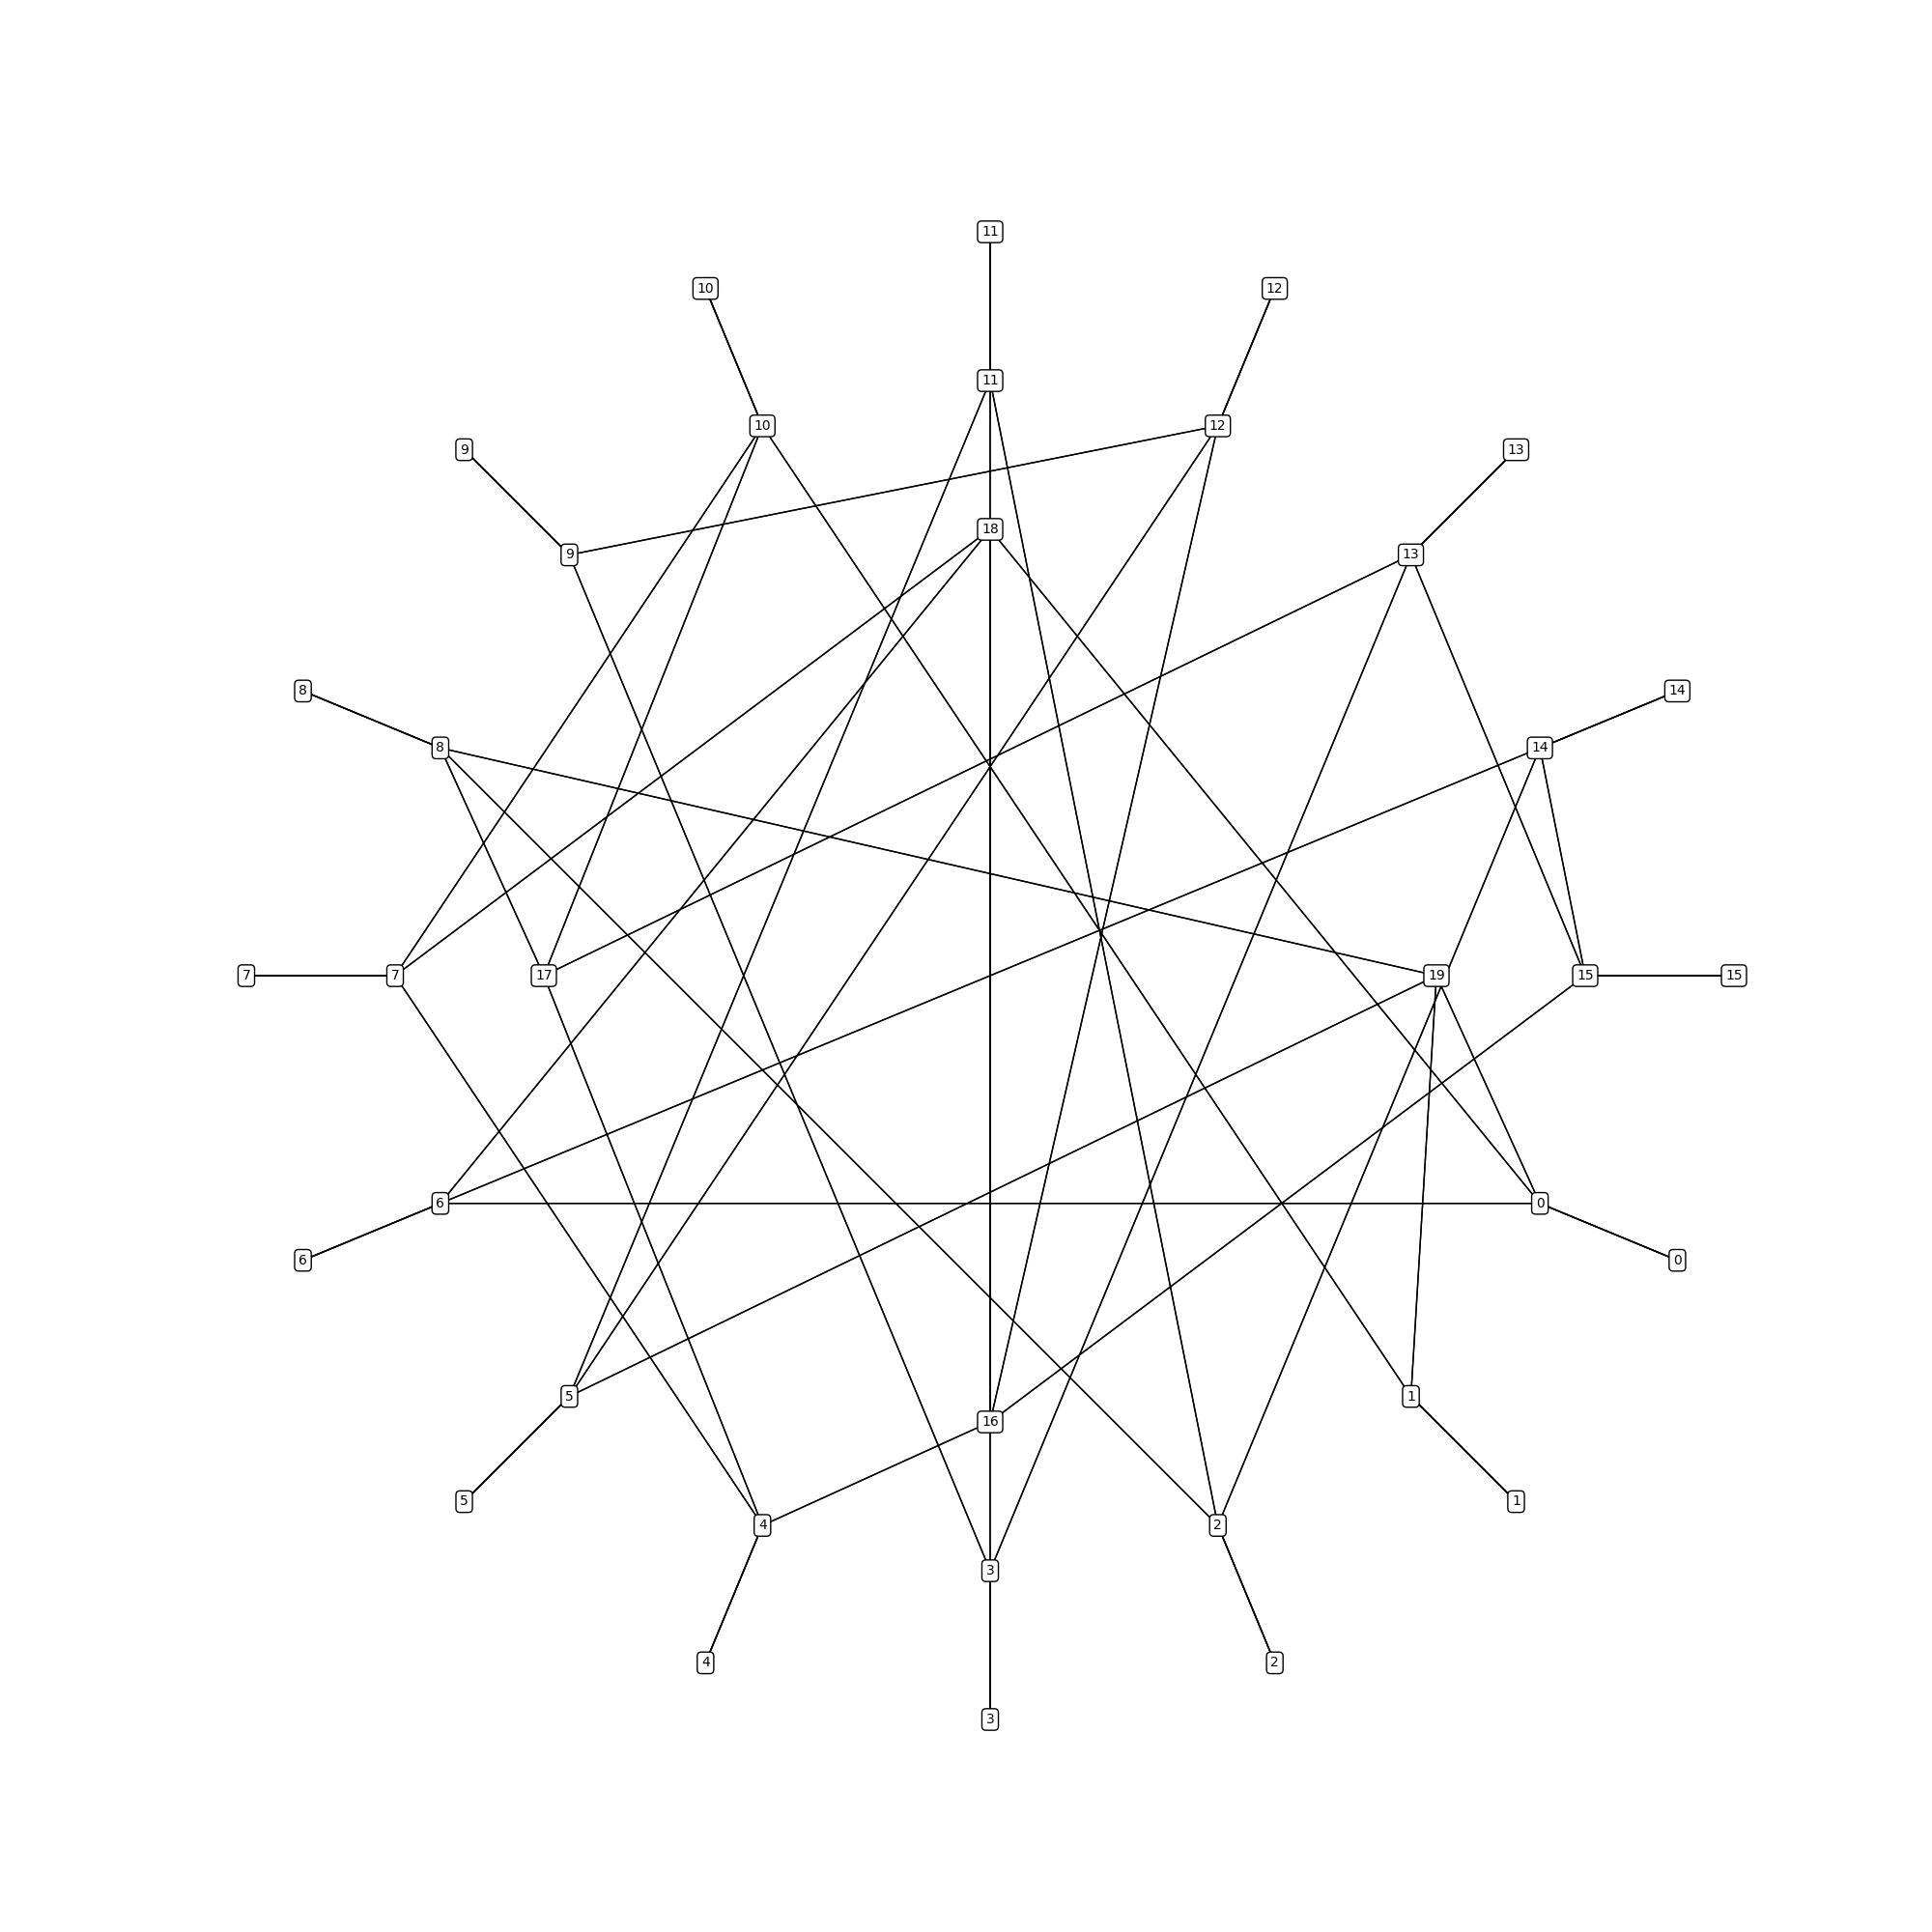
\includegraphics[scale=0.35]{acn/lab2/figures/plot_jellyfish_4.png}
    \caption{Jellyfish with 4 ports}
    \label{fig:jelly6}
\end{figure}

\newpage


\section{Comparing the Properties of Fat-tree and Jellyfish}

% Start your writing here, feel free to include subsections to structure your report if needed
% Please remove the note below in your submission


\subsection{Running the Code}

\subsubsection{Figure 1c}
\textbf{Prerequisites:} matplotlib, numpy, networkx\\
\textbf{Execution:} python3 reproduce\_1c.py\\
\textbf{Disclaimer:} This took $\approx$10 minutes for 14 ports, 686 servers, 245 switches and 10 iterations for the jellyfish topology

\subsubsection{Figure 9}
\textbf{Prerequisites:} matplotlib, numpy, pathos\\
\textbf{Execution:} python3 reproduce\_9.py\\
\textbf{Disclaimer:} This took $\approx$1.5hours with 8 thread for 14 ports, 686 servers and 245 switches, only works on Linux due to some recursion limits with Pickle

\subsection{General approach}

\subsubsection{Figure 1c}

To calculate the distribution of the path lengths for Jellyfish and Fat-tree we followed this process:
\begin{enumerate}
    \item generating a Fat-tree topology and using our own implementation of Dijkstra to calculate all shortest paths
    \item calculating the distribution of these path lengths for Fat-tree for paths with length 2 to 6
    \item generating 10 Jellyfish topologies and using Dijkstra again to calculate all shortest paths
    \item calculating the distribution of the paths with length 2 to 6 for Jellyfish averaging over all 10 runs
\end{enumerate}

Plotting the results is done with matplotlib by creating a bar chart.


\subsubsection{Figure 9}

We implemented \textit{Yen's Algorithm} close to the provided Wikipedia pseudo-code.
Furthermore we added some conditions wich allowed the algorithm to finished after only 8 paths if there are no shorter paths available (therefore we have alle the paths we need for 8 shortest, ECMP 8-Way and ECMP 64-Way).
After getting the needed paths we calculate the how often each link appears in every path.
Last but not least we calculate the ranks for every number of distinct links and plot the figure with the obtained data.

We initially thought we would need to permutate all the servers which leads to a much higher execution time.
After looking at the figure and analysing our differences to the original figure we would have taken a different approach (s. \autoref{sec:reproduce:discussion}).

\subsection{Reproduced Figures}

\subsubsection{Figure 1c}

The figure 1c is very similar to the original figure in the paper.
The small differences are discussed in \autoref{sec:reproduce:discussion}.

\begin{figure}[ht]
    \centering
    \includegraphics[scale=0.5]{acn/lab2/figures/fig_1c.png}
    \caption{Figure 1c reproduced}
    \label{fig:jelly6}
\end{figure}

\subsection{Figure 9}
\label{sec:reproduce:fig9}
The figure 9 looks a little bit different.
Please read in the discussion (s. \autoref{sec:reproduce:discussion}) why we think that happened.

\begin{figure}[ht]
    \centering
    \includegraphics[scale=0.75]{acn/lab2/figures/fig_9.png}
    \caption{Figure 9 reproduced}
    \label{fig:jelly6}
\end{figure}

\newpage

\subsection{Discussion}
\label{sec:reproduce:discussion}

\subsubsection{Figure 1c}

For the bars of the fat-tree there is no visible difference which makes sense due to the statically defined nature of the topology.
The jellyfish results are a little bit different for paths with length 2 and 3 this could happen due to the way we distribute the servers to the switches (dividing the servers by the switches and rounding up).

\subsubsection{Figure 9}
Figure 9 looks different because we run the Yen's algorithm for 686 different permutations for all the servers.
We figure that the original paper uses permutation for switches because the servers actually do not matter for the Yen algorithm because it will always be the same links.
We suspect that the paper did 1000 iterations with different switch permutations which lead to higher rank of links for a smaller number of distinct paths.
However, our figure still represents the same claim of the paper that using the 8 shortest paths is more beneficial than ECMP.

\section{Bonus}
% Start your writing here for the bonus part
% Please remove this section if you are not attempting the bonus


\subsection{Running the Code}

\textbf{Prerequisites:} matplotlib, numpy, networkx, pathos\\
\textbf{Execution:} python3 reproduce\_9bcube.py or python3 reproduce\_9dcell.py\\
\textbf{Disclaimer:} This took $\approx$30 minutes for 25 ports (\textit{DCell}) and 512 server with 8 levels (\textit{BCube}).

\subsection{General Approach for Topologies}
We implemented \textit{DCell}\footnote{Chuanxiong Guo, Haitao Wu, Kun Tan, Lei Shi, Yongguang Zhang, Songwu Lu. DCell:A Scalable and Fault-Tolerant Network Structure for Data Centers. ACM SIGCOMM 2008.} and \textit{BCube}\footnote{Chuanxiong Guo, Guohan Lu, Dan Li, Haitao Wu, Xuan Zhang, Yunfeng Shi, Chen Tian, Yongguang Zhang, Songwu Lu, Guohan Lv. BCube: A High Performance, Server-centric Network Architecture for Modular Data Centers. ACM SIGCOMM 2009.} closely to the provided papers.

\subsubsection{BCube}
Normally the BCube would need two inputs - n, the number of servers per BCube\_0 and k, the levels.
However, we wanted to keep using the same kind of inputs with num\_ports and num\_servers which is why there are some limitations to the input.
If a input is wrong the next correct possible input is chosen and a error message is displayed.
The implementation itself is relatively short and follows the paper closely.
First all the server are created with appropriate names.
Then we iterate over the number of levels for the BCube and generate the switches per level.
Those switches are then connected to the required servers.

\begin{figure}[ht]
    \centering
    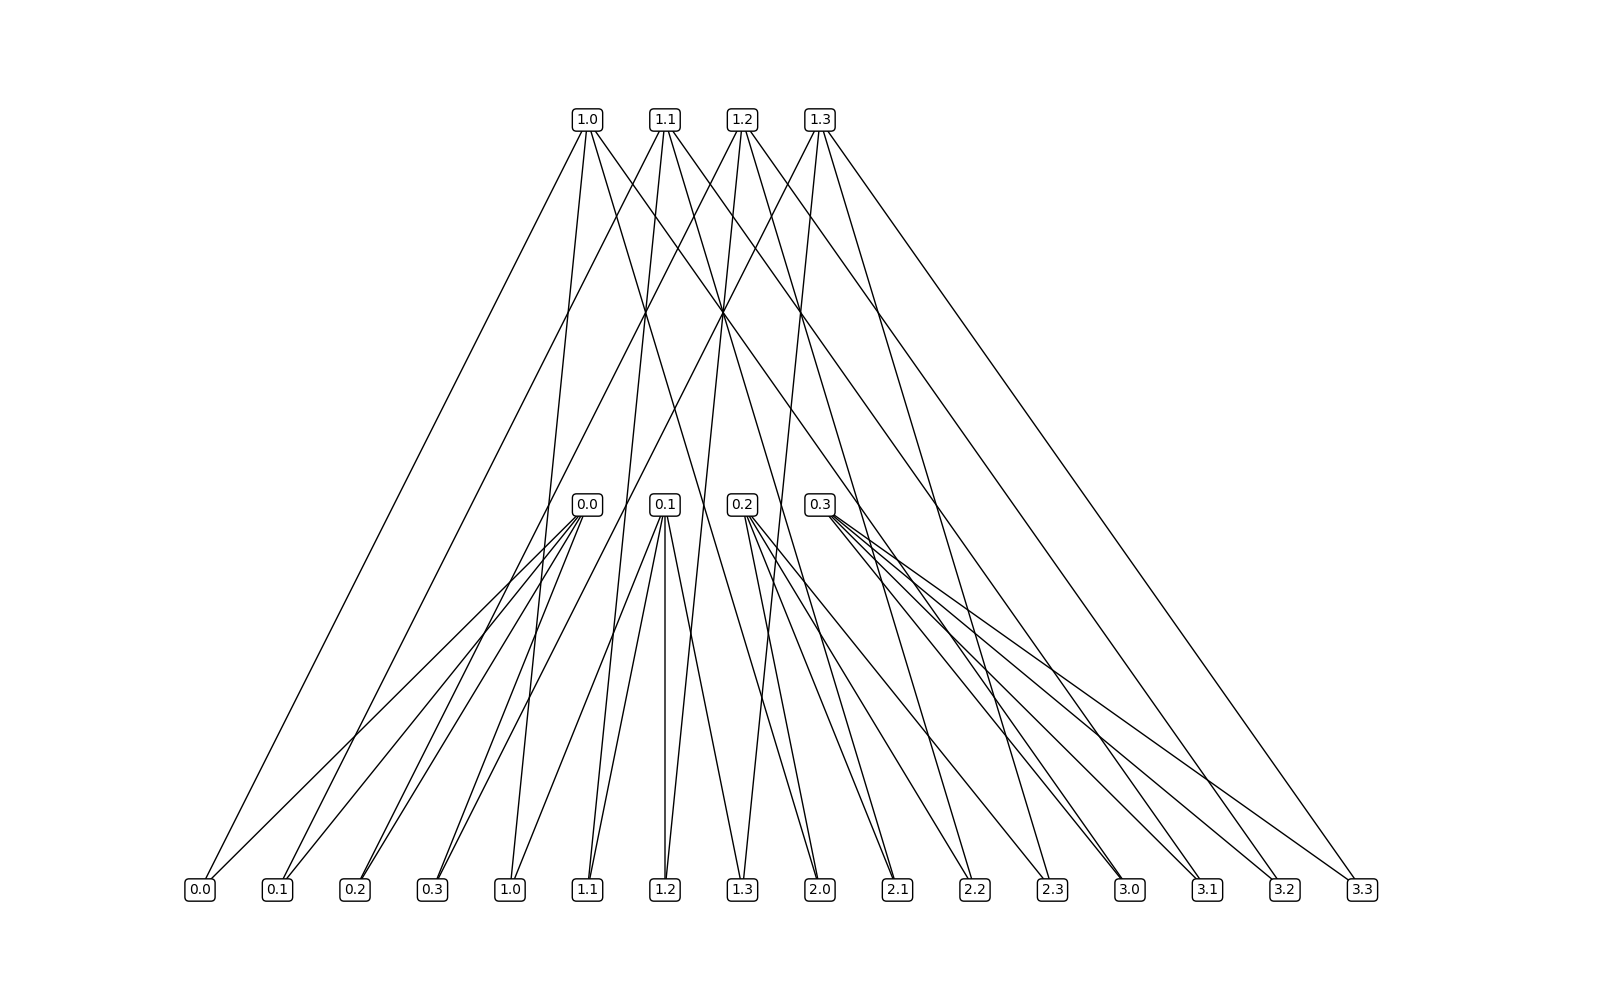
\includegraphics[scale=0.3]{acn/lab2/figures/plot_bcube_16.png}
    \caption{Topology for \textit{BCube} with 4 ports and 16 servers}
    \label{fig:topo_dcell}
\end{figure}

\subsubsection{DCell}
For DCell just the number of ports ($n$) is relevant since we assume it equals the number of servers.
A network using \textit{DCell} is able to support $n \cdot (n + 1)$ servers.
Therefore, a \textit{DCell0} has a miniswitch and $n$ connected servers.
To generate a \textit{DCell1}, a topology of level 1 containing $n$-times $+1$ \textit{DCell0}s, we used the recursive approach described in the paper.
After setting up the relevant \textit{DCell0}s we just have to connect the servers of the first \textit{DCell0} to all other \textit{DCell0}s.
From there on we keep connecting the other servers of the \textit{DCell0}s until all \textit{DCell0}s are interconnected.
At the moment we just support \textit{DCell}s with level 1.
Even after a lot of research we were not able to get it running and did not find a single implementation which supports higher levels than 1 in a recursive manner.
But you can simply use more than 14 ports.
To compare the topologies we took 25 ports in account which gives us a total number of $25\cdot (25 +1)= 650$ connectable servers for our \textit{DCell} implementation.

\begin{figure}[ht]
    \centering
    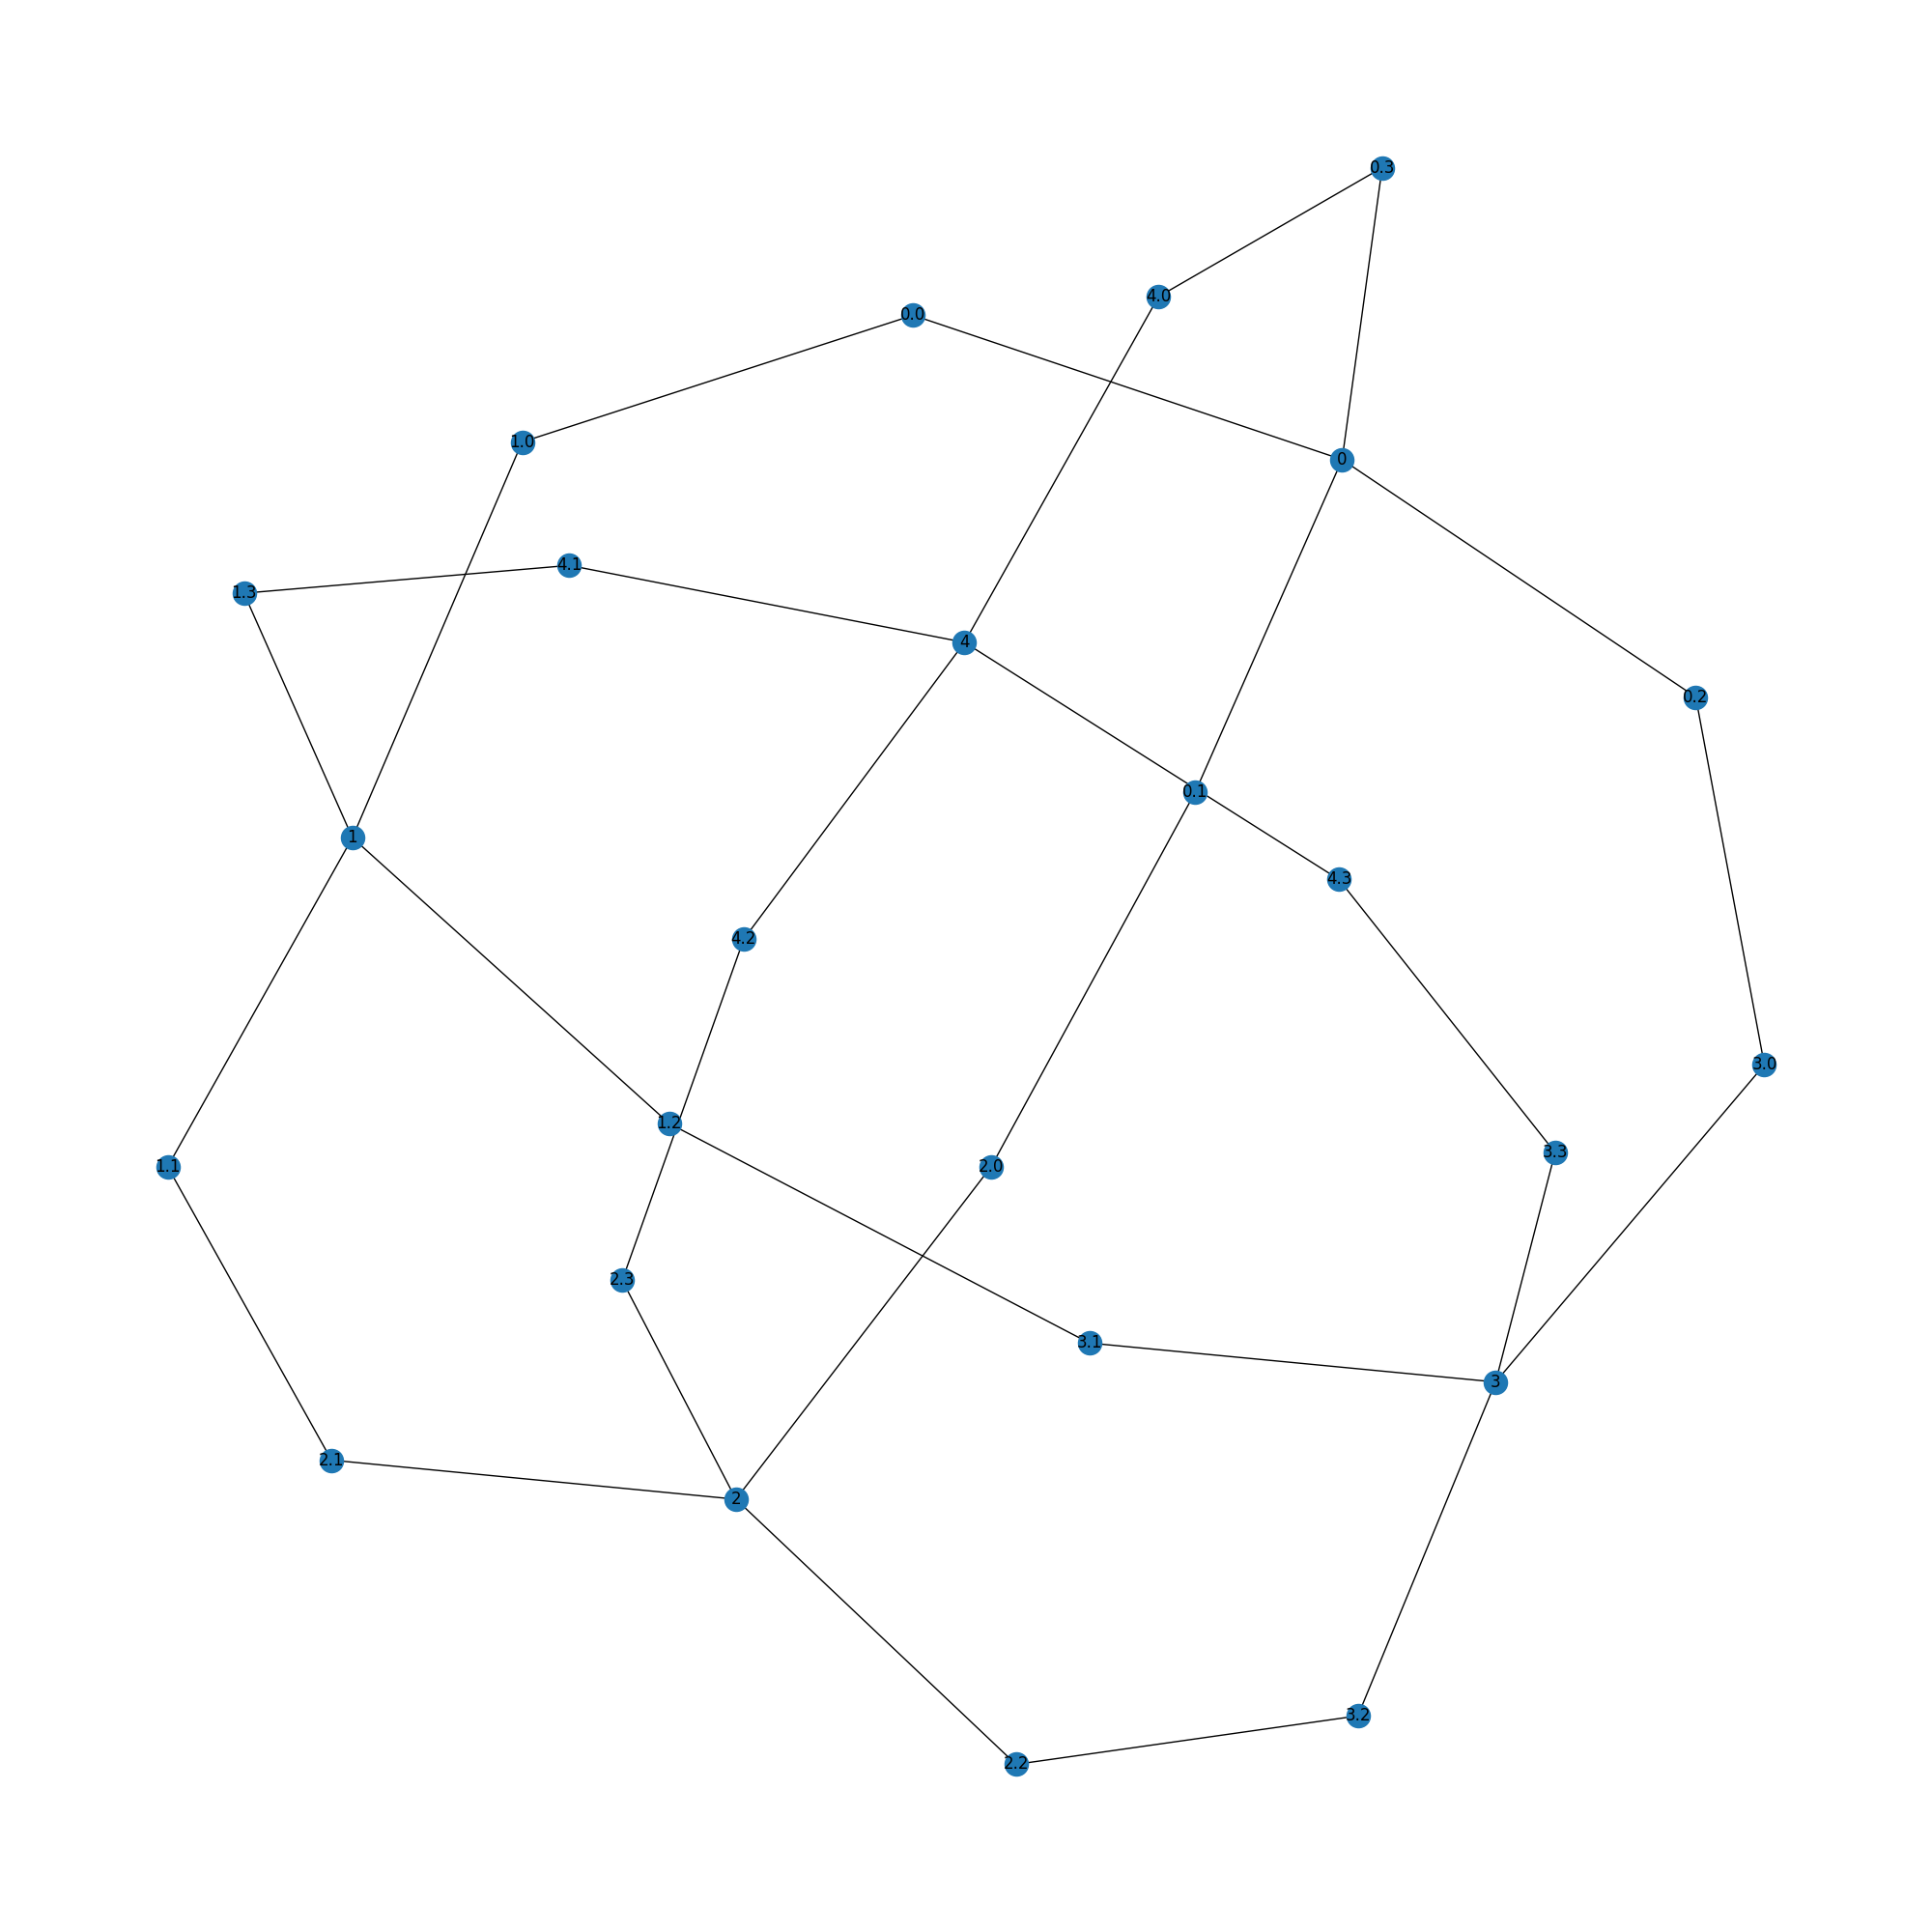
\includegraphics[scale=0.3]{acn/lab2/figures/plot_dcell_4.png}
    \caption{Topology for \textit{DCell} with 4 ports and 20 servers}
    \label{fig:topo_dcell}
\end{figure}

\subsection{Reproduced Figures}

\subsubsection{BCube}
s. \autoref{fig:fig_9_bcube}
\begin{figure}[ht]
    \centering
    \includegraphics[scale=0.75]{acn/lab2/figures/fig_9_bcube.png}
    \caption{Figure 9 \textit{BCube} with 512 server and 8 levels}
    \label{fig:fig_9_bcube}
\end{figure}

\subsubsection{Dcell}
s. \autoref{fig:fig_9_dcell}

\begin{figure}[ht]
    \centering
    \includegraphics[scale=0.75]{acn/lab2/figures/fig_9_dcell.png}
    \caption{Figure 9 \textit{DCell} with 25 ports and 650 servers}
    \label{fig:fig_9_dcell}
\end{figure}

\subsection{Discussion}

It is obvious that the figures 9 with BCube and DCell do not look like the one from Jellyfish.
However, it is still visible that the same claim from the Jellyfish Topology (using 8-Shortest-Path) is still the best option for BCube as well as DCell.

Furthermore we can observe that there is a extreme discrepancy between the 8-Shortest-Path and ECMP for DCell for the number of distinct links.

\end{document}

